% =====================================================================
%  Malaria detection -- working manuscript template (Science Fair, FJFI CTU)
%
%  This is a DRAFT. It describes the CURRENT solution (ResNet50 + k-NN baseline).
%  Rewrite the parts marked "For the team:" to match YOUR own solution
%  (different classifier, different features, better results).
%
%  Compile: pdfLaTeX + BibTeX  (Overleaf does this automatically).
% =====================================================================
\documentclass[11pt]{article}

\usepackage[utf8]{inputenc}
\usepackage[T1]{fontenc}
\usepackage[english]{babel}
\usepackage{lmodern}

\usepackage{amsmath}
\usepackage{booktabs}
\usepackage{siunitx}
\usepackage{graphicx}
\usepackage{xcolor}
\usepackage[margin=2.5cm]{geometry}
\usepackage[colorlinks=true,allcolors=blue]{hyperref}
\usepackage[capitalize,nameinlink]{cleveref}

\sisetup{detect-weight=true, table-number-alignment=center}

% --- Measured values (k-NN baseline, test set). The team replaces these. ---
\newcommand{\Ntotal}{27\,558}
\newcommand{\Ntrain}{19\,289}
\newcommand{\Nval}{4\,135}
\newcommand{\Ntest}{4\,134}
\newcommand{\knnK}{31}
\newcommand{\knnAcc}{0.77}      % accuracy at threshold 0.5
\newcommand{\knnSens}{0.56}     % sensitivity at threshold 0.5
\newcommand{\knnSpec}{0.99}     % specificity at threshold 0.5
\newcommand{\knnFN}{904}        % missed sick cells at threshold 0.5
\newcommand{\knnTP}{1163}
\newcommand{\knnSpecNF}{0.00}   % COMPETITION metric: specificity @ sensitivity >= 99 %
\newcommand{\knnAUC}{0.93}

\title{\textbf{Detecting the Malaria Parasite in Blood Smears with\\
Transfer Learning and $k$-Nearest Neighbours}\\[4pt]
\large\textnormal{Working manuscript template --- adapt it to your own solution}}

% For the team: fill in your names and team name.
\author{First Last \and First Last\\[2pt]
\small Team ``\dots'' \,$\cdot$\, Science Fair \,$\cdot$\, Department of Mathematics, FJFI CTU}
\date{\today}

\begin{document}
\maketitle

\begin{abstract}
\noindent
Malaria kills roughly 600{,}000 people every year, mostly where trained pathologists able to
recognise the parasite under a microscope are scarce. We study whether this task can be
automated: on a public dataset of \Ntotal{} microscopy images of individual red blood cells
(National Institutes of Health, NIH) we distinguish healthy cells from cells infected by the
\emph{Plasmodium} parasite. Our current solution first uses a frozen ResNet50 convolutional
neural network as a feature extractor and then classifies the resulting vectors with a simple
$k$-nearest-neighbours ($k$-NN) rule. This baseline reaches an area under the ROC curve of
\knnAUC{} on the test set. At the same time we show why accuracy alone is misleading in
medicine: at the default decision threshold the model attains an accuracy of \knnAcc{} but a
sensitivity of only \knnSens{}, missing nearly half of the infected cells. This document is a
starting point; you replace it with your own, stronger classifier at the marked places.
\end{abstract}

% =====================================================================
\section{Introduction and Problem Statement}
\label{sec:intro}

Malaria remains one of the deadliest infectious diseases: according to the World Health
Organization (WHO), about 600{,}000 people died of it in 2022~\cite{who2023}. Reliable
diagnosis still relies on the so-called thick drop and thin blood smear, where a technician
searches red blood cells under a microscope for the \emph{Plasmodium} parasite. This procedure
is slow, requires an experienced specialist, and precisely in the regions with the highest
malaria burden such specialists are critically scarce. This raises the question we address:
\emph{can the decision ``is this cell infected?'' be reliably delegated to an algorithm?}

The key obstacle for classical machine learning is that training an image recogniser from
scratch requires millions of labelled images and substantial computing power. We sidestep both
through \emph{transfer learning}: we take a network pre-trained on millions of ordinary
photographs, reuse its ability to ``see'' shapes and textures, and only re-train a small
decision part. Concretely, in this draft we combine a frozen ResNet50 feature extractor with a
$k$-nearest-neighbours classifier and reach an area under the ROC curve of \knnAUC{} on the NIH
dataset; at the same time we stress that the quality of a medical classifier must be judged by
its sensitivity and specificity, not by accuracy alone.

This document is a \textbf{working template}. It describes the baseline solution and its
evaluation so that you can start from it and replace it with your own, improved approach. The
places where you should do so are marked ``For the team''.

\medskip\noindent\textit{For the team: add one sentence here stating how your solution differs
from the baseline and what main result it achieves.}

% =====================================================================
\section{Data}
\label{sec:data}

We use the public \emph{Malaria Cell Images} dataset from the U.S. National Institutes of
Health~\cite{rajaraman2018}. It contains \Ntotal{} colour images of individual, already
segmented red blood cells and is perfectly \emph{balanced} --- exactly half of the cells are
infected and half are healthy (13{,}779 and 13{,}779). The balance matters for interpreting the
results: it means that random guessing yields 50~\% accuracy, so any improvement above this line
comes from a genuinely learned distinction.

To make the results an honest measure of generalisation to new cells, we split the data into
three parts in a \emph{stratified} way (preserving the class ratio) and with a fixed random
seed: a training set (\Ntrain{} cells), a validation set (\Nval{} cells) for tuning and model
selection, and a held-out test set (\Ntest{} cells) used exclusively for the final evaluation.
A separate test set is essential: without it we could easily tune the model to the specific data
and overestimate its true quality.

% =====================================================================
\section{Method}
\label{sec:method}

\subsection{Feature extraction with a frozen ResNet50}
\label{sec:features}

Because we have neither enough data nor time to train a convolutional neural network (CNN) from
scratch, we use the ResNet50 network~\cite{he2016} pre-trained on the ImageNet dataset as a
\emph{feature extractor}. We first apply standard preprocessing to each cell image (resizing to
224$\times$224 pixels and colour normalisation as expected by ImageNet) and then pass it through
the network with its final classification layer removed. The output for each cell is a vector of
\textbf{2048 numbers} --- the \emph{features}, which summarise what is in the image (shapes,
textures, spots). We keep the network \emph{frozen}: its weights do not learn, it merely
translates an image into numbers. This reduces the whole task to classifying vectors, which even
a weak computer handles in a few seconds.

\subsection{Classification with $k$-nearest neighbours}
\label{sec:knn}

As the initial classifier we deliberately chose the simplest possible model in order to obtain
an honest \emph{baseline} for comparison: the $k$-nearest-neighbours ($k$-NN)
rule~\cite{cover1967}. It does not actually train --- it merely memorises the training features.
It classifies a new cell by finding the $k$ closest (most similar in feature space) among the
memorised cells and letting them vote, with nearer neighbours weighted more heavily; the
fraction of votes for the class ``infected'' is taken as the estimated probability. We used
$k=\knnK{}$ neighbours and standardised the features before computing distances (zero mean, unit
variance), because distances are only meaningful when the individual features share a comparable
scale.

\medskip\noindent\textit{For the team: this is where you replace \cref{sec:knn} with your own
solution --- for example a small trained neural network. Describe its architecture and how you
tuned it.}

% =====================================================================
\section{Evaluation}
\label{sec:eval}

\subsection{Why accuracy alone is not enough}
\label{sec:metrics}

In medicine the two kinds of error carry very different costs, which is why we do not measure a
classifier's quality by \emph{accuracy} (the fraction of correctly classified cells) alone. Let
us denote as true positive (TP) an infected cell correctly flagged, false negative (FN) an
infected cell wrongly declared healthy, false positive (FP) a healthy cell wrongly flagged as
infected, and true negative (TN) a healthy cell correctly passed. From these we define two key
quantities:
%
\begin{equation}
\mathrm{sensitivity} = \frac{\mathrm{TP}}{\mathrm{TP}+\mathrm{FN}}, \qquad
\mathrm{specificity} = \frac{\mathrm{TN}}{\mathrm{TN}+\mathrm{FP}}\,.
\label{eq:senspec}
\end{equation}
%
Sensitivity says what fraction of the truly sick the model catches; low sensitivity means missed
patients, which can cost a life. Specificity says what fraction of the healthy the model
correctly passes; low specificity means needless false alarms. These two quantities trade off
against each other depending on the chosen \emph{threshold} above which a cell is declared
infected; the whole trade-off is captured by the ROC curve (receiver operating characteristic)
and summarised by the area under it (area under the curve, AUC).

As the main \textbf{competition metric} we chose the \emph{specificity at a sensitivity of
$\geq 99~\%$}. For a deadly disease the non-negotiable requirement is ``not missing a sick
patient'', so we fix sensitivity high (catch at least 99~\% of the infected) and compete on who
keeps the highest specificity, that is the fewest false alarms. This corresponds to the point on
the ROC curve at a sensitivity of 99~\%.

\subsection{Protocol}
\label{sec:protocol}

We ``train'' the classifier (for $k$-NN, merely memorise) on the training set, perform any
threshold selection on the validation set, and measure all numbers reported below on the
held-out test set (\Ntest{} cells), which the model never sees during learning. The $k$-NN
method is deterministic, so we report the results of a single run.

\subsection{Results}
\label{sec:results}

The baseline results are summarised in \cref{tab:results}. The most telling point is the
conflict between accuracy and sensitivity: at the default threshold of $0.5$ the $k$-NN reaches
an accuracy of \knnAcc{} but a sensitivity of only \knnSens{} --- as the confusion matrix in
\cref{fig:confusion} shows, it misses \knnFN{} of the 2067 infected cells. The high specificity
(\knnSpec{}) thus masks the fact that the model passes nearly half of the sick; accuracy alone
would have deceived us. The full ROC curve (\cref{fig:roc}) shows that the \emph{ranking} ability
is not bad: the area under it is \knnAUC{}. Our competition metric is stricter, however. We
require catching at least 99~\% of the sick, and under this constraint the specificity of $k$-NN
drops to \knnSpecNF{} --- to catch 99~\% of the infected it would have to push the threshold so
low that it flags nearly every cell. The $k$-NN therefore does satisfy the required sensitivity,
but only at essentially zero specificity --- practically useless; this is exactly why a learned
model is needed (your task).

% --- Results table -----------------------------------------------------
\begin{table}[t]
\centering
\caption{Results on the held-out test set (\Ntest{} cells). Accuracy, sensitivity and
specificity are reported at the default threshold $0.5$; the competition metric is the
specificity at a sensitivity of $\geq 99~\%$. Values are from a single deterministic run.}
\label{tab:results}
\begin{tabular}{l S[table-format=1.2] S[table-format=1.2] S[table-format=1.2] S[table-format=1.2] S[table-format=1.2]}
\toprule
Method & {Accuracy} & {Sensitivity} & {Specificity} & {Spec.\,@\,sens.\,99\,\%} & {AUC} \\
\midrule
ResNet50 + $k$-NN (baseline) & 0.77 & 0.56 & 0.99 & 0.00 & 0.93 \\
Your solution                & {--} & {--} & {--} & {--} & {--} \\
\bottomrule
\end{tabular}
\end{table}

% --- Figures -----------------------------------------------------------
\begin{figure}[t]
\centering
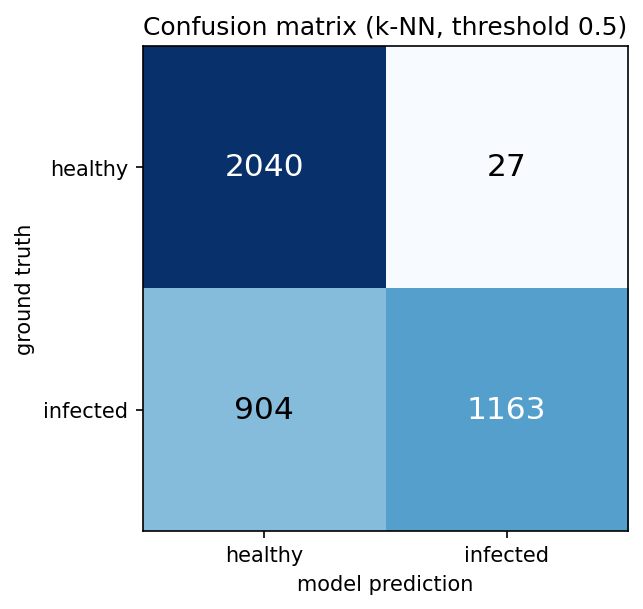
\includegraphics[width=0.55\linewidth]{figs/confusion_baseline_en.png}
\caption{Confusion matrix of the $k$-NN baseline on the test set at threshold $0.5$. Rows are
the true classes, columns the predictions. The bottom-right cell (\knnTP{}) are correctly caught
sick cells, the bottom-left cell (\knnFN{}) are \emph{missed} sick cells --- the most expensive
type of error.}
\label{fig:confusion}
\end{figure}

\begin{figure}[t]
\centering
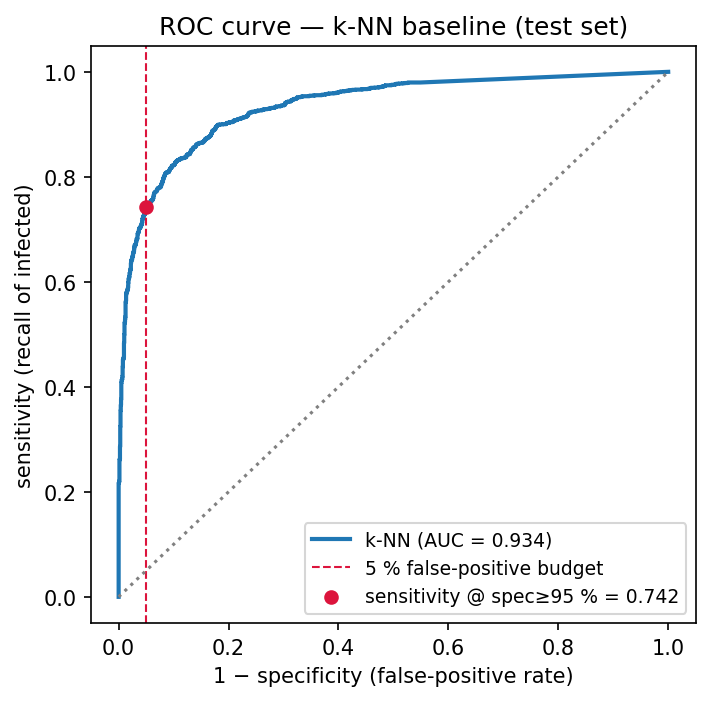
\includegraphics[width=0.6\linewidth]{figs/roc_baseline_en.png}
\caption{ROC curve of the $k$-NN baseline on the test set. The horizontal line marks the
required sensitivity of 99~\%; the competition metric is the highest specificity attainable above
that line. The baseline only reaches it at a near-100~\% false-positive rate (specificity $\approx 0$).}
\label{fig:roc}
\end{figure}

% =====================================================================
\section{Discussion}
\label{sec:discussion}

The weaker $k$-NN result is not an accident but a consequence of two effects worth noting. First,
in the 2048-dimensional feature space distances stop being informative --- all points become
roughly equidistant, so the notion of a ``nearest neighbour'' loses its sharpness (the
\emph{curse of dimensionality}). Second, $k$-NN learns nothing: it cannot weigh which of the 2048
features matter for telling the parasite apart, treating them all equally. This is exactly where
a better-informed model that learns what matters has room to improve.

Independently of the model used, two practical limitations remain. A real deployment would face
\emph{domain shift} --- a different microscope, different staining, or a different patient
population could lower the accuracy relative to our dataset. And because the cost of a missed
sick patient exceeds the cost of a false alarm, in practice the model is better suited as a tool
that \emph{flags} cases for a clinician than as a final arbiter.

\medskip\noindent\textit{For the team: this is where the analysis of your results belongs --- what
worked, what did not, by how much you beat the baseline, and how you explain it.}

% =====================================================================
\section{Conclusion}
\label{sec:conclusion}

We have shown that a frozen ResNet50 used as a feature extractor, combined with a simple
$k$-nearest-neighbours classifier, reaches an area under the ROC curve of \knnAUC{} on the NIH
dataset, and we have stressed why medicine requires judging sensitivity and specificity rather
than accuracy alone. This baseline is the starting point your solution is meant to beat ---
in particular by keeping the specificity as high as possible at the required sensitivity of 99~\%.

% =====================================================================
% Bibliography lives in refs.bib.
% Compile with BibTeX: pdflatex -> bibtex -> pdflatex -> pdflatex
\bibliographystyle{unsrt}
\bibliography{refs}

\end{document}
